\subsection{Windsimulation}

\subsubsection{Allgemeines}

Für die Simulation des Winds ist es wichtig, eine möglichst optimale
Datenstruktur zur Speicherung der verwendeten Felder zu verwenden, um
die Speicherzugriffszeiten zu minimieren und die maximale Performance zu
erreichen.

Wie bereits angesprochen bietet OpenCL zur Speicherung die Wahl zwischen Buffern
und Texturen (sofern Texturen auf der Zielplattform unterstützt werden). Beide
Speicher-Arten haben leicht unterschiedliche Anwendungsgebiete. In vielen
Kerneln sind wir daran interessiert, für die \PimiddyQuotes{aktuelle} Zelle den
Wert des Gitters sowie den Wert aller Nachbarn zu bestimmen, wobei der
\PimiddyQuotes{Wert} je nach Feld-Typ entweder Druck, Geschwindigkeit oder etwas
anderes bedeuten kann. Außerdem wird bei der Advektion linear zwischen Voxeln
interpoliert.

Schnelle Zugriffe auf einen Voxel samt seiner Nachbarn sind ein Merkmal von
Texturen, daher würden sie sich für viele Kernel anbieten. Allerdings ist das
Schreiben von 3D-Texturen in OpenCL-1.1 nur mit einer Extension möglich. Als
Hilfsmaßnahme greift man hier üblicherweise zu sogenannten
\PimiddyBegriff{Flat-3D-Texturen} \cite{Harris2003}. Hier werden die einzelnen
\PimiddyQuotes{Scheiben} der dreidimensionalen Struktur nebeneinander in eine
zweidimensionale Textur geschrieben, siehe
\autoref{fig:implementation_flat_3d_texture}. Für die Umrechung zwischen 3D- und
2D-Koordinaten ist etwas Rechenaufwand nötig. 2D-Texturen erlauben außerdem
natürlicherweise nur zweidimensionale Interpolation. Benötigt man
dreidimensionale Interpolation, ist auch hier etwas Mehraufwand zu verrechnen.
Texturen werden optimiert gespeichert, sodass Leseoperationen beschleunigt
werden. Diese optimierte Speicherung führt aber dazu, dass das Schreiben in
Texturen relativ langsam ist. Benchmarks im Zweidimensionalen bestätigten, dass
Buffer tatsächlich schneller sind.

\begin{figure}[ht]
\centering
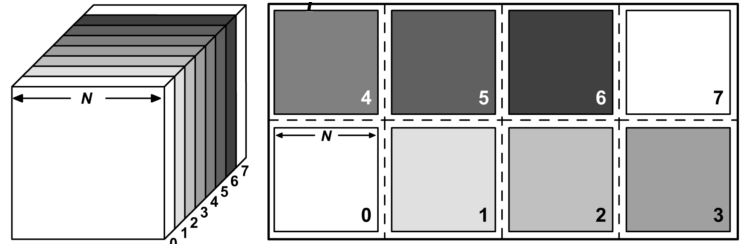
\includegraphics[width=10cm]{images/flat_3d_texture}
\caption{Veranschaulichung einer Flat-3D-Textur}
\label{fig:implementation_flat_3d_texture}
\end{figure}

Da Buffer eindimensional sind, muss zwischen drei- und eindimensionalen
Koordinaten konvertiert werden. Sei $(x,y,z)$ eine dreidimensionale Koordinate
und $(w,h,d)$ die Dimensionen eines Buffers (er enthält also $w \cdot h \cdot d$
Elemente). Dann erhält man den eindimensionalen Index mittels:

\begin{equation}
i = w \cdot h \cdot z + w \cdot y + x
\end{equation}

Umgekehrt erhält man die $(x,y,z)$-Koordinaten eines Index mittels

\begin{align*}
x &= i \PimiddyModulo w \\
y &= i \PimiddyModulo w \cdot h \\
z &= i / (w \cdot h)  \\
\end{align*}

Im Weiteren wird das Verfahren von Stam in OpenCL umgesetzt. Dabei wird auf
Besonderheiten in der Implementierung eingegangen. Fast alle Kernel greifen
hierbei auf den Buffer zurück, der die Hindernisinformationen enthält. Wie
dieser Buffer gefüllt wird, wird im letzten Abschnitt erläutert.

\subsubsection{Verfahren nach Stam in OpenCL}

Es sollen nun die einzelnen Schritte des Verfahrens in OpenCL-Kernel umgewandelt
werden, wobei an einigen Stellen auf Details verzichtet wird. Der Teil des
Programms, der auf dem Host läuft, soll hier ebenfalls nicht in Gänze erarbeitet
werden. Stattdessen soll deutlich werden, in welcher Reihenfolge die Kernel
aufgerufen werden und welche Daten beim Aufruf gelesen und geschrieben werden.
Aus Einrückungsgründen werden viele Bezeichner abgekürzt, aber immer so, dass aus
der Erläuterung bzw\,. den Kommentaren noch hervorgeht, was sich dahinter
verbirgt.

Die Simulation benötigt einige persistente Daten Daten, also solche, die
zwischen den Simulationsschritten beibehalten werden und nicht nur temporär für
berechnungen verwendet werden:

\begin{itemize}
\item ein Buffer \PimiddyInlineCode{boundaries} vom Typ
\PimiddyInlineCode{float}, der 1.0 enthält, wenn die zugehörige Gitterzelle ein
Hindernis enthält und 0.0 wenn nicht. Das Befüllen dieses Buffers wird in
Abschnitt xxx beschrieben.
\item ein Buffer \PimiddyInlineCode{velocity} vom Typ
\PimiddyInlineCode{float4}, der das momentane Geschwindigkeitsfeld enthält.
Dieses Feld wird anfangs auf $(0,0,0,0)$ gesetzt. Der Wind wird manuell von
einer Seite in die Simulation gespeist und breitet sich dann aus.
\item Viele der Algorithmen benötigen außerdem das aktuelle Zeitdelta
\PimiddyInlineCode{float dt}, was die Zeit seit dem letzten Simulationsdurchlauf
angibt.
\end{itemize}

\begin{figure}[ht]
\centering
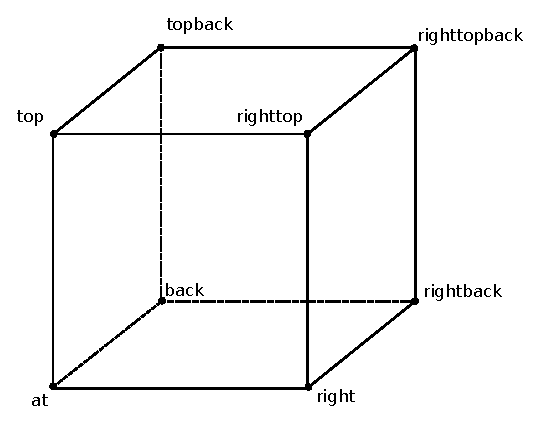
\includegraphics[width=10cm]{images/right_neighborhood}
\caption{Veranschaulichung der Nachbarschaftsstruktur \PimiddyInlineCode{neighbors}}
\label{fig:implementation_right_neighbors}
\end{figure}

Die meisten Kernel werden mit einer dreidimensionalen Arbeitsgröße initialisiert
und müssen auf den aktuellen Voxel, sowie seine Nachbarn zugreifen. Daher bietet
es sich an, den Übergang von einem drei- zu einem eindimensionalen Index in eine
Funktion auszulagern. Diese Funktion kann gleichzeitig testen, ob ein gegebener
Index den Rand des Gitters verlässt, und in dem Fall den nächstbesseren Voxel am
Rand zurückliefern. Diese Funktion \PimiddyInlineCode{i4p} ist im Folgenden
dargestellt:

\begin{minted}[frame=lines]{c}
// Bekommt die Gittergroesse s und eine 3D-Position p.
// Liefert einen Index.
uint i4p(uint3 p,uint3 s)
{
    // Komponentenweise in gueltigen
    // Bereich [0,n-1] transformieren
    p = clamp(p,(uint3)(0,0,0),s - (uint3)(1,1,1));
    return s.w * s.h * p.z + s.w * p.y + p.x;
}
\end{minted}

Der erste Schritt im Verfahren von Stam ist die Advektion des Vektorfeldes
\PimiddyInlineCode{velocity}. Der dazugehörige Kernel ist in mehreren Funktionen
und Strukturen aufgeteilt, die nun im einzelnen erklärt werden sollen.

Man benötigt zunächst eine Struktur, um einen Geschwindigkeitswert sowie die direkten
Nachbarn zu speichern (siehe \autoref{fig:implementation_right_neighbors}).

\begin{minted}[frame=lines]{c}
typedef struct neighbors
{
    float3 at;
    float3 right,top,back,righttop;
    float3 rightback,topback;
    float3 righttopback;
};
\end{minted}

Diese Struktur wird von einer zugehörigen Funktion zurückgegeben, die eine
beliebige Position im Gitter sowie die Größe des Gitters als Eingabe bekommt:

\begin{minted}[frame=lines]{c}
// Parameter genau wie i4p, zusaetzlich
// noch "b"
neighbors neighbors_for_pos(
    global float4 *b,
    uint3 p,
    uint3 s)
{
    neighbors result;
    result.at = b[i4p(p,s)];
    result.right = b[i4p(p+(uint3)(1,0,0),s)];
    result.top = b[i4p(p+(uint3)(0,1,0),s)];
    result.back = b[i4p(p+(uint3)(0,0,1),s)];
    result.righttop = b[i4p(p+(uint3)(0,1,1),s)];
    result.rightback = b[i4p(p+(uint3)(1,0,1),s)];
    result.topback = b[i4p(p+(uint3)(0,1,1),s)];
    result.righttopback = b[i4p(p+(uint3)(1,1,1),s)];
    return result;
}
\end{minted}

Schließlich wollen wir mit Hilfe dieser Nachbarstruktur einen interpolierten
Vektor erzeugen. Hier hilft die Funktion \PimiddyInlineCode{mix}, die linear
zwischen zwei Werten anhand eines dritten Wertes interpoliert:

\begin{minted}[frame=lines]{c}
float3 interpolate_neighbors(
    neighbors n,
    // v ist ein Vektor im Intervall [0,1]
    float3 v)
{
    float3
            v1 = mix(
                    mix(n.at ,n.right ,v.x),
                    mix (n.top ,n.righttop ,v.x),
                    v.y),
            v2 = mix(
                    mix(n.back ,n.rightback ,v.x),
                    mix(n.topback ,n. righttopback ,v.x),
                    v.y);

    return mix(v1,v2,v.z);
}
\end{minted}

Der eigentliche Kernel hat schließlich folgende Form:

\begin{minted}[frame=lines]{c}
kernel void advection(
    global float *boundary,
    global float3 *input,
    global float3 *output,
    float dt,
    uint3 size)
{
    uint3 position = (int3)(
            get_global_id(0),
            get_global_id(1),
            get_global_id(2));

    uint index = i4p(position);

    if(boundary[index] > 0.5f)
    {
            output[index] = (float3)(0.0f);
            return;
    }

    float4
            v = input[index],
            advected = convert_float3(position) - dt * v,
            fractions = fract(advected_vector);

    neighbors n = neighbors_for_pos(
            input,
            position,
            size);

    output[index] = interpolate_neighbors(
            n,
            fractions);
}
\end{minted}

ür den Projektionsschritt benötigen wir die Divergenz des Vektorfeldes.
Analog zur Advektion definieren wir eine Struktur, um die Von Neumann-
Nachbarschaft eines Gitterpunktes zu speichern:

\begin{minted}[frame=lines]{c}
typedef struct vn_neighbors
{
    float4 at;
    float4 left, right;
    float4 top, bottom;
    float4 front, back;
    float boundary_at;
    float boundary_left, boundary_right;
    float boundary_top, boundary_bottom;
    float boundary_front, boundary_back;
};
\end{minted}

Die Struktur enthält zusätzlich noch die zu den Nachbarn gehörigen Hin-
derniswerte, die Bestimmung dieser Werte und die der Vektoren verläuft aber
nach demselben Schema wie bei der Advektion und sei im Folgenden mit
\PimiddyInlineCode{vn\_neighbors\_for\_pos(...)} bezeichnet.
Bei der Bestimmung der Divergenz müssen die Randbedingungen beachtet werden. Ist
einer der Nachbarn von einem Hindernis ausgefüllt, wird statt des Vektors an
dieser Stelle der Nullvektor angenommen. Statt dies jedoch als eine womöglich
aufwändige Bedingung umzusetzen kann stattdessen erneut dieFunktion mix
verwendet werden, wobei als Interpolationsparameter direkt der Hinderniswert
eingesetzt wird. Der zur Divergenz gehörige Kernel sieht so aus:

\begin{minted}[frame=lines]{c}
kernel void divergence(
    global float4 *input,
    global float *output,
    global float *boundary,
    uint3 size)
{
    uint4 position = (int3)(
            get_global_id(0),
            get_global_id(1),
            get_global_id(2));

    uint index = i4p(position);

    vn_neighbors n = vn_neighbors_for_pos(
            input,
            position,
            boundary,
            size);

    float3 z = (float3)(0.0f);

    n. left = mix(n.left, z, n.boundary_left);
    n. right = mix(n.right, z, n.boundary_right);
    n.top = mix(n.top, z, n.boundary_top);
    n. bottom = mix(n.bottom, z, n.boundary_bottom);
    n. front = mix(n.front, z, n.boundary_front);
    n. back = mix(n.back, z, n.boundary_back);

    output[index] =
            (n.right - n.left).x +
            (n.bottom - n.top).y +
            (n.front - n.back).z;
}
\end{minted}

\begin{itemize}
\item Dann Jacobiverfahren, hier vor allem Pingpong zwischen Buffern erklären
und wie viele Iterationen man machen muss/kann.
\item Dann Subtraktion des Gradienten
\item Hindernisse, Visualisierung (Laden aus obj-Datei)
\item Hindernisse, Voxelisierung mit binvox (Quelle \cite{Nooruddin2003}, \cite{binvox2012}
\end{itemize}